\section{Background}
\label{sec:background}
Despite recent interest, concerns about system power have existed since the dawn of computing. Some of the earliest valve-based computers had power draws comparable to modern supercomputers. The ENIAC machine dissipated 174 kW \cite{birnbaum:2000aa}, a figure which would not look out of place in the current Top 500 list, despite the fact this machine dates from 1947.\golden

When bipolar semiconductor technologies superseded thermionic valves in the 1950s and 60s there was a dramatic reduction in system power consumption. Over time, manufacturing improvements delivered ever smaller transistors, yielding rapid increases in both performance and power density. Ultimately this resulted in escalating power draws which strained the limits of cooling technologies~\cite{jouppi:1994aa}. \golden

The use of bipolar semiconductors peaked in the early 1990s when they were replaced in turn with the more efficient Complementary Metal Oxide Semiconductor (CMOS) technology we still rely on today. CMOS was a mature technology which offered far superior energy consumption characteristics. It had been  overlooked previously as it was thought to be too slow for use in high-performance microprocessors. \golden

\begin{figure}[ht]
\centering
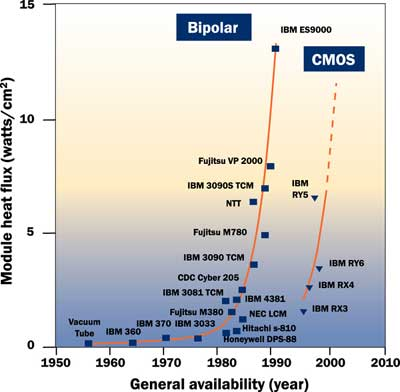
\includegraphics[width=0.9\linewidth]{Images/bipolarcmos.jpg}
\caption{Trends in module level power density, reproduced from \cite{chu:1999aa}. Copyright 1999 IEEE.}
\end{figure}
This pattern of improving hardware until physical limits force a switch to new technologies is a recurring one. The previous iteration saw the widespread adoption of multi-core architectures, and once again we find ourselves encountering fundamental limitations \cite{esmaeilzadeh:2011aa}. Unfortunately,  this time there are no mature semiconductor technology or transformational architectural paradigm waiting in the wings. Researchers are therefore searching for alternative ways to combat the rise of power consumption whilst we await the emergence of the next fundamental shift in processor technology. \golden

System architects are already focussing on power efficient chip design, with recent innovations in areas including on-die voltage regulation \cite{burton:2014aa}, Dynamic Voltage and Frequency Scaling (DVFS) scheduling \cite{kwon:2013aa} and energy efficient heterogeneous cores~\cite{gupta:2012aa}. Software engineers are also beginning take note of this issue as it becomes an increasingly pressing concern for scientific computing. \golden

The power draw of CMOS chips can be split into distinct components, the most significant of which are dynamic power and leakage power. Dynamic power is essentially the power consumed as logic gates change state while a processor performs work. Leakage power dissipation stems from the fact that at very small scales the insulating properties of silicon break down, allowing some current to flow even when gates remain inactive. Other forms of power dissipation exist, however their effects are relatively minor. \golden

\begin{equation}
\label{eq:totpwr}
P_{tot} = P_{dyn} + P_{leak} + P_{other}
\end{equation}
\begin{equation} 
\label{eq:dynpwr}
P_{dyn} \propto CV^{2}Af
\end{equation}
\begin{equation}
\label{eq:leakpwr}
P_{leak} \propto V\left(ke^{\frac{-qV_{th}}{ak_{a}T}}\right)
\end{equation}

Equations~\ref{eq:dynpwr} and \ref{eq:leakpwr} above give relations for dynamic and sub-threshold leakage power respectively. In Equation~\ref{eq:dynpwr}, C denotes load capacitance (a property influenced by wire lengths of on-chip structures), $V$ the supply voltage, $A$ the activity factor and $f$ the clock frequency. Most of these terms are properties of the processor itself, however $A$ loosely equates to processor workload. Finally, the $V$ and $f$ terms are linked and vary in tandem as higher clock frequencies require higher supply voltages to sustain them. \golden

Equation~\ref{eq:leakpwr} is a simplified equation for sub-threshold leakage power. The new terms introduced in this equation include $T$, temperature, $V_{th}$, the transistor threshold voltage and $k$ the Boltzmann constant. The remaining parameters $q$, $a$ and $k_{a}$ capture CMOS logic design and fabrication characteristics. This is only one of several kinds of power leakage, however they all share the fact that they do not directly depend on processor workload. This means they are out of scope for software optimization and their details can be omitted.

Historically, dynamic power has been the biggest contributor to $P_{tot}$, however leakage power has been on track to overtake it since the breakdown of Dennard Scaling.  Sub-threshold and gate-oxide leakage dominate total leakage current, with both increasing exponentially as transistors shrink. Process improvements like the introduction of high-k dielectric materials~\cite{jan:2009aa} have kept leakage power in check over the last decade, however there is no avoiding the fact that insulating properties will degrade as transistors get smaller. \golden

An important feature of the equations governing power draw is that only $P_{dyn}$ is directly influenced by software, in particular due to its inclusion of the $A$ term. Software can also indirectly effect both dynamic and leakage current if it triggers changes to clock frequency and therefore supply voltage through DVFS. \golden

The final things we must consider are the metrics which can be used when optimizing for energy consumption. Energy to completion is one obvious choice which is widely used in domains where available energy is severely limited. That said, the fact that it fails to capture runtime restricts its usefulness and has led in turn to the development of other more comprehensive metrics.

In practice, the metrics chosen are those which  combine the effects of both energy and runtime. The simplest of these is the energy-delay product (EDP) \cite{gonzales:1995aa}, which assigns an equal weighting to both runtime and energy consumption. EDP can be defined in various equivalent ways:\golden

\begin{equation}
EDP = Energy \times Runtime
\end{equation}
\begin{equation}
\label{eq:edp}
EDP = Power \times Runtime^{2}
\end{equation}
\begin{equation}
EDP = Power \times (Instructions / MIPS)^{2}
\end{equation}

Several variants of EDP have been proposed which assign greater weight to the runtime component in accordance with the demands of high performance computing. Common examples include energy-delay-squared product ($ED^{2}P$) and energy-delay-cubed product ($ED^{3}P$). We refer to this as the $E^mD^n$ family of metrics, which also includes simple power ($E^1D^{-1}$), energy ($E^1D^0$) and time ($E^0D^1$) as members. It can be argued that that $ED^{2}P$ is most suited when considering a fixed micro-architecture \cite{brooks:2000aa}, however our work applies to all members of this group where $M > 0$.